\section{Methods}

    This section provides a comprehensive overview of the methodologies employed in various stages of our research. These stages are i) collection of beer microbiome data samples; ii) implementation, evaluation, and automation of bioinformatics analysis workflows for the data and reproducibility analysis; and iii) the construction of the beer microbiome database, BeerMicroDB, which was designed to serve as a comprehensive overview of beer microbiome data and the reproduced results using the workflows created. 
    
    \subsection{Data collection}

        In the beginning, due to uncertainty about the adequacy of beer-related data samples, the decision was made to collect samples not only of beer but also of cider, Kombucha, kefir, and wine. The procedure for data collection was bifurcated. The first avenue involved seeking out research articles on the microbiome of fermented drinks via Google Scholar. The availability of public sample data was then verified for each paper. If such data was available, it was added to a spreadsheet along with relevant metadata. The second method involved a direct search for microbiome samples related to fermented drinks in databases such as ENA or MG-RAST \cite{keegan2016mg}. Any suitable datasets found this way were also added to the spreadsheet. In total, 768 samples were collected.
        
        Once data collection was completed, the Python libraries \tool{pandas} and \tool{matplotlib} were used in a \tool{Jupyter Notebook} to graphically represent the data, facilitating a preliminary understanding of its composition.

        \begin{figure}[H]
            \centering
            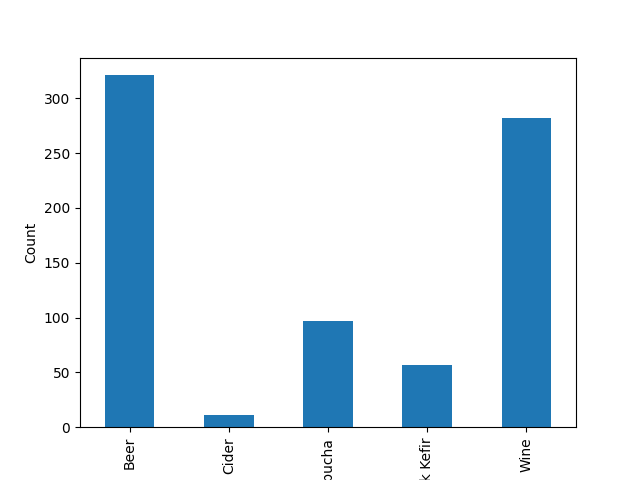
\includegraphics[scale=0.5]{images/methods/data_composition_by_type.png}
            \caption{Overview of fermented drinks}
            \label{fig:methods:data_composition_by_type}
            \small Number of data samples by fermented drink types, which consist of Beer, Cider, Kombucha, Milk Kafir, and Wine.
        \end{figure}

        To deepen our understanding of the collected data, we first examine the number of samples associated with each type of fermented drink shown in figure \ref{fig:methods:data_composition_by_type}. Subsequently, to enhance our insight, we explore how these samples are distributed across various extraction techniques, such as shotgun and metabarcoding techniques. For the metabarcoding approach, we pay special attention to the distribution of sequencing targets, including but not limited to ITS and 16S shown in figure \ref{fig:metabarcoding_data}.

        \begin{figure}[H]
             \centering
             \begin{subfigure}[b]{0.45\textwidth}
                \centering
                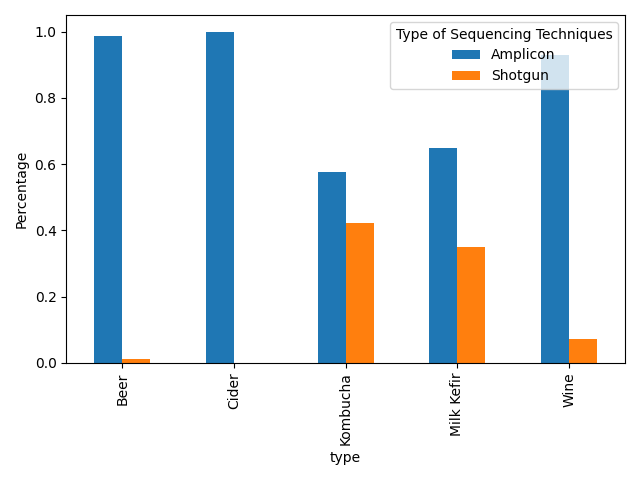
\includegraphics[scale=0.5]{images/methods/data_composition_by_sequencing_techniques.png}
                \caption{Data composition by sequencing techniques}
                \label{fig:methods:data_composition_by_sequencing_techniques}
             \end{subfigure}
             \hfill
             \begin{subfigure}[b]{0.45\textwidth}
                \centering
                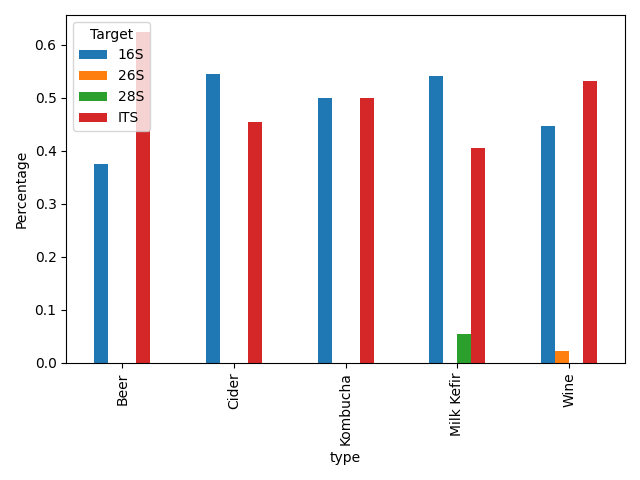
\includegraphics[scale=0.5]{images/methods/metabarcoding_data_composition_by_targets.png}
                \caption{Metabarcoding data composition by targets}
                \label{fig:methods:metabarcoding_data_composition_by_targets}
             \end{subfigure}
                \caption{Data composition by sequencing techniques and metabarcoding targets}
                \label{fig:metabarcoding_data}
        \end{figure}

        Through meticulous data collection, we have assembled a substantial array of beer samples. Our observation indicates that the majority (higher than 95\%) of our metabarcoding data  can be categorized as either ITS or 16S.  The beer sample did not even have 26S and 28S data. With this in mind, and given the adequate amount of data for the beer samples, which is over 300, we have chosen to focus only on these beer samples at the moment.

        While we're concentrating on beer samples now, we're open to the prospect of incorporating data on other fermented drink types in the future. Our current database comprises 317 beer samples. We found that a small subset of these samples (16 to be precise) are housed on the MG-RAST platform, in the form of FASTA files, while all other data samples are in the form of FASTQ files, for keeping consistency, we decided to omit these from our immediate analysis.
        
        In conclusion, our study will concentrate on the remaining 301 beer samples. The volume of data contained within these samples establishes a robust foundation for our continuing investigations. We have made the scripts for plotting the figures, as well as information about the datasets, accessible to the public. These resources can be accessed at the following URL: \url{https://github.com/asdsd/sdfdfs/blob/main/data_plot_n_processing/data_plot.ipynb}.

    
    \subsection{Microbiome analysis workflows}

        This section shows the implementation and evaluation of the workflows used in the thesis and also the methodologies and tools used in the reproducibility analysis.
        
        \subsubsection{Implementation of workflows}

        This section illustrates the implementation of metabarcoding and shotgun workflows accordingly.
        
        \subsubsection*{Metabarcoding workflow}
            Based on the characteristics and comparison of state-of-the-art tools for analyzing metabarcoding data discussed in the section "State of the art: Data Analysis" we use QIIME 2 as the workflow for analyzing metabarcoding data.

        \paragraph*{QIIME 2 Set up on Galaxy Europe}
            QIIME 2 was available as 109 Galaxy wrappers and initially not available on Galaxy Europe and therefore needed to be installed. This involved extracting the QIIME 2 Galaxy tools from the qiime2/galaxy-tools GitHub repository, which contains Official QIIME 2 tools for Galaxy, by using scripts designed to extract all tool IDs into a YAML file and subsequently merging them into the usegalaxy-eu/usegalaxy-eu-tools repository.
        
        After completing this process, the QIIME 2 tools can be accessed through the Galaxy Europe instance. However, to ensure that these tools are executed using docker when invoked, the associated tool IDs must also be added to the job\_conf.yml file in the usegalaxy-eu/infrastructure-playbook repository.
        
        Thus, with the above procedure, the QIIME 2 tools have been successfully configured on the Galaxy Europe instance. The scripts for setting up QIIME 2 on Galaxy Europe can be accessed at the following URL: \url{https://github.com/YedilSerzhan/beer_microbiome/tree/main/qiime2_tools_crawler}.

        \begin{figure}[H]
            \centering
            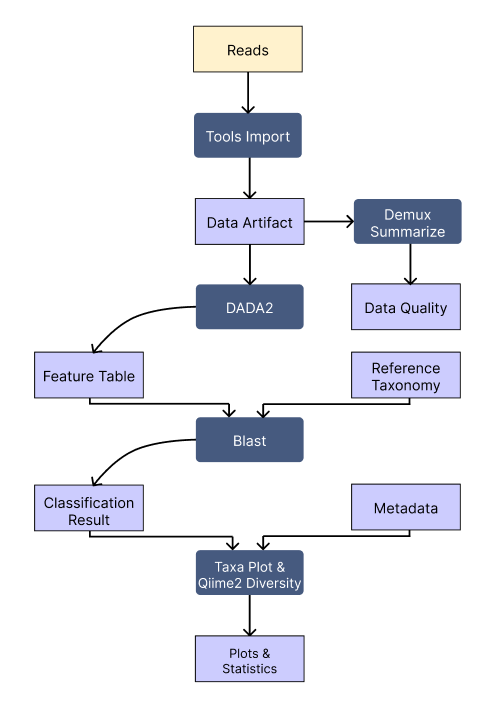
\includegraphics[scale=0.5]{images/metabarcoding_workflow.png}
            \caption{The metabarcoding workflow}
            \small The metabarcoding workflow is implemented using QIIME 2. The steps contain data importing, DADA 2 denoising, taxonomy profiling using BLAST, and visualization \& diversity analysis. (Elements with dark blue color are for tools and purple color are for results of the intermediate steps)
            \label{fig:methods:amplicon_workflow}
        \end{figure}
            
        \paragraph*{Data importing}
            Firstly data files from ENA should be uploaded to Galaxy using the upload function. However, all QIIME 2 tools interact with artifacts instead of traditional data files like FASTQ or FASTA files. A QIIME 2 artifact is a file with .qza extension. In order to convert the input data to an artifact, the tool \tool{qiime2 tools import} needs to be used. There is one parameter "Type of data to import" that needs to be set. For a FASTQ data file, we should choose the "SampleData[PairedEndSequencesWithQuality]" option. Then we need to specify the data file and the file format to import from. Normally in the QIIME 2 CLI version, we can choose the files and format by creating a manifest file, which declares the name and location of each data file to be imported. However, in Galaxy, the location of uploaded data files can't be accessed for security reasons. So in QIIME 2 Galaxy version, we can do it by choosing the option "Casava One Eight Single Lane Per Sample Directory Format" and renaming each data file to the format like "L2S357\_15\_L001\_R1\_001.fastq.gz".The underscore-separated fields in this file name are (1) the sample identifier (2) the barcode sequence or a barcode identifier (3) the lane number (4) the direction of the read (i.e. only R1, because these are single-end reads) and (5) the set number. This certainly has set some limitations for the variety of types of data to process, for example, FASTA files can not be properly processed using QIIME 2 Galaxy.


        \paragraph*{Quality control and feature table construction}

            After importing the data, the quality of the data can be accessed using the tool \tool{qiime2 demux summarize}, which can provide an interactive plot of the quality of the data. Next depending on the data quality information, parts of the data can be truncated or trimmed. 

            The quality control and amplicon sequence variant (ASV) feature table construction can be done using the tools \tool{DADA2}. Deblue is also available for feature table construction but it needs additional quality filtering steps, so dada2 is chosen here. Rather than adopting the conventional approach of "OTU-picking" that is commonly used in metabarcoding workflows, DADA2 \cite{callahan2016dada2} introduces a unique algorithm that simulates the inaccuracies generated in the course of metabarcoding. By employing this error model, the algorithm can deduce the actual composition of a sample. It generates tables of amplicon sequence variants (ASVs), which provide a higher level of resolution in comparison to traditional methods. Based on whether the data is paired or not,  \tool{qiime2 dada2 denoise-single} or \tool{qiime2 dada2 denoise-paired} will be used.
            
            \textbf{Options:}
                For DADA2 denoising, depending on the quality of the data, a few parameters can be set: 1. "trunc\_len": Position at which sequences should be truncated due to a decrease in quality. 2."trim\_left": Position at which sequences should be trimmed due to low quality  3. "max\_ee": Reads with a number of expected errors higher than this value will be discarded. This procedure takes normally around 10 minutes depending on the size of the data. These options should be set depending on the quality information gotten from the result of \tool{qiime2 demux summarize}. 
            
            \textbf{Outputs:}
                The outputs consist of 3 files. 1. "feature table": The resulting feature table is a tabular representation of the data that maps samples to ASVs.  2. "representative sequences": The resulting feature sequences. Each feature in the feature table will be represented by exactly one sequence. 3. "denoising stats": stats about the denoising procedure like how many reads are removed, the percentage of reads that are preserved, and so on. This information can help you have an understanding of how well the denoising is conducted and whether you want to change the parameters and do it again.
    
            \textbf{Visualization for outputs:}
                In order to view the output results, we can use the following tools. For a feature table, we can use \tool{qiime2 feature-table summarize} to generate visual and tabular summaries of a feature table. For the denoising stats, we can use \tool{qiime2 metadata tabulate} to generate a visualization that shows a tabular view of data. And it supports interactive filtering, sorting, and exporting to common file formats.


        \paragraph*{Taxonomy profiling}
            In this step, we’ll perform annotation of the features that were observed in the last denoising step by performing taxonomic classification of the sequences. The tool used in the workflow is \tool{qiime2 feature-classifier classify-consensus-blast}, the function of which is assigning taxonomy to query sequences using BLAST+. Performs BLAST+ local alignment between query and reference reads, then assigns consensus taxonomy to each query sequence from among max accepts hits, min consensus of which share that taxonomic assignment.
    
            \textbf{Inputs and reference database:}
            The required inputs for this tool are  1. Query sequences. 2. Reference sequences. and 3. reference taxonomy labels. The query sequences come from the output representative sequences of DADA 2 denoising. The reference sequences and reference taxonomy labels come from a reference database that we can choose. Until now, for QIIME 2, the available options are UNITE for fungal ITS, Silva for 16S/18S rRNA, and Greengenes for 16S rRNA. In our case, we stick to UNITE for fungal ITS and Silva for 16S rRNA.  

            \textbf{Optional parameters:}
            There are 4 important optional parameters that can be set for consensus-blast. (1) maxaccepts: the maximum number of hits to keep for each query. The first N hits will be chosen in the reference database that is similar to the query the default value is 10. (2) perc\_identity: A float number from 0.0 to 1.0 to reject a match if the percent identity to query is lower. The default value is 0.8. (3) query-cov: A float number from 0.0 to 1.0 with a default value of 0.8. The algorithm rejects matches if query alignment coverage per high-scoring pair is lower than this value. (4) min-consensus: A float number ranging from 0.5 to 1.0 represents the minimum fraction of assignments that must match the top hit to be accepted as consensus assignments. The default value is 0.51. Throughout the processing of all data, most of them are set to use the default values.

            \textbf{Algorithm outputs:}
            There are 2 outputs generated in the end. They are classification and search results. The classification file is the taxonomy classifications of query sequences. And the search results file shows the top hits for each query.

                Both files can be visualized using the \tool{qiime2 feature-table summarize} tool.


        \paragraph*{Diversity analysis and visualization}
            For a more comprehensive grasp of the results, we can employ diversity analysis to assess the richness and diversity within and among the samples. The use of visualization tools can further enhance our insight into the results, offering a more detailed and intuitive understanding of the data.

            There are 2 tools that can be used to do the diversity analysis. The tool \tool{qiime2 diversity alpha} is for computing a user-specified alpha diversity metric for all samples in a feature table. And tool \tool{qiime2 diversity beta} can be used to compute a user-specified beta diversity metric for all pairs of samples in a feature table. The input is the feature table generated by the dada2-denoising tool. And we can choose a metric out of dozens of options.

            Apart from visualizing the intermediate results from the previous steps using tools \tool{qiime2 metadata tabulate} and \tool{qiime2 feature-table summarize}. We can also use \tool{qiime2 taxa barplot} to generate an interactive bar chart visualizing the taxonomic classification results. 

                The inputs are (1) Feature table: the feature table generated by the DADA2 denoising tool. And (2) Taxonomy: Taxonomic annotations for features in the provided feature table, which is the file generated by the tool \tool{qiime2 feature-classifier classify-consensus-blast}.

                The output file is a barplot.qzv file which can be visualized using the QIIME 2 View website to generate an interactive bar chart plot can include multi-level sorting from level 1 kingdom to level 7 species, plot recoloring, sample relabeling, and SVG figure export. If a proper metadata file is also provided as input, you can also group and sort by the metadata columns. 

        
        \subsubsection*{Shotgun workflow}
        
            As we transition to the more comprehensive shotgun sequencing approach, which indiscriminately sequences all the DNA within a sample, we are met with a change in both the scope and the complexity of the analysis. Consequently, the workflow for shotgun sequencing requires a shift in the analytical tools and methods employed. This section talks about the workflow implementation for shotgun data.
            
        \paragraph*{Existing workflow}

            There is already a Galaxy tutorial available on workflows on identifying beer micro-organisms before this thesis (\url{https://training.galaxyproject.org/training-material/topics/metagenomics/tutorials/beer-data-analysis/tutorial.html}).
                        
            \begin{figure}[H]
                \centering
                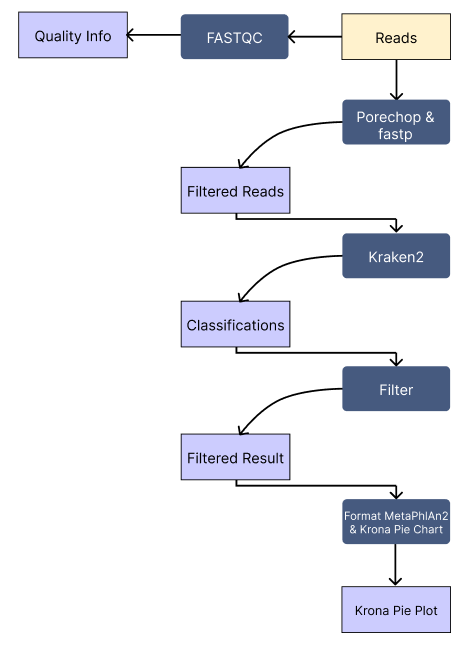
\includegraphics[scale=0.5]{images/existing_shotgun_workflow.png}
                \caption{The existing shotgun workflow}
                \small The existing workflow initiates with quality control measures employing tools such as FASTQC, Oirechop, and fastp. Subsequently, taxonomic profiling is undertaken using Kraken 2. Once profiled, the filtered results are visualized utilizing the Format MetaPhAn2 and Krona Pie charts.
                \label{fig:methods:existing_shotgun_workflow}
            \end{figure}

            The established workflow illustrated in figure \ref{fig:methods:existing_shotgun_workflow} begins with the utilization of \tool{FASTQC} \cite{andrews2010fastqc} to evaluate the quality of the reads. The resulting HTML file vividly portrays the quality scores distributed over all bases. \tool{Porechop} \cite{wick2017completing} is subsequently employed to eliminate sequencing adapters and chimeras, or contaminants. Moreover, the tool \tool{fastp} \cite{chen2018fastp} aids in filtering sequences possessing low-quality scores. One can review the HTML report generated by \tool{fastp} to ascertain how the data quality has been enhanced.

            The subsequent step is taxonomic classification, for which we utilize \tool{Kraken2}. The database incorporated in this phase is the "Prebuilt Refseq indexes: PlusPF". If the "Create Report" option in Kraken2 is selected, a report file encompassing detailed information is produced. The report's first column displays clades, extending from taxonomic domains (like Bacteria, Archaea, and so forth) to species. The second column discloses the number of reads allocated to the clade rooted at that particular taxon.
            
            For visualizing the results, we employ \tool{MetaPhlAn2}  \cite{blanco2023extending} to transfigure the report into the Krona format. Subsequently, the \tool{Krona pie chart} tool can process the converted report file to construct a Krona pie chart. This chart is a multilayered pie chart that exhibits the community profile. The central part of the chart represents higher taxonomy levels (such as the domain), whereas the outer parts provide more detailed information (such as species).
            
        \paragraph*{Updates to the shotgun workflow}

            The existing workflow for shotgun sequencing analysis has been in place for an extended period. During this time, there have been significant updates to both the tools and databases involved in the process. Notably, the advent of the Kraken software suite \cite{lu2022metagenome} has necessitated further updates to the shotgun workflow.

            \begin{figure}[H]
                \centering
                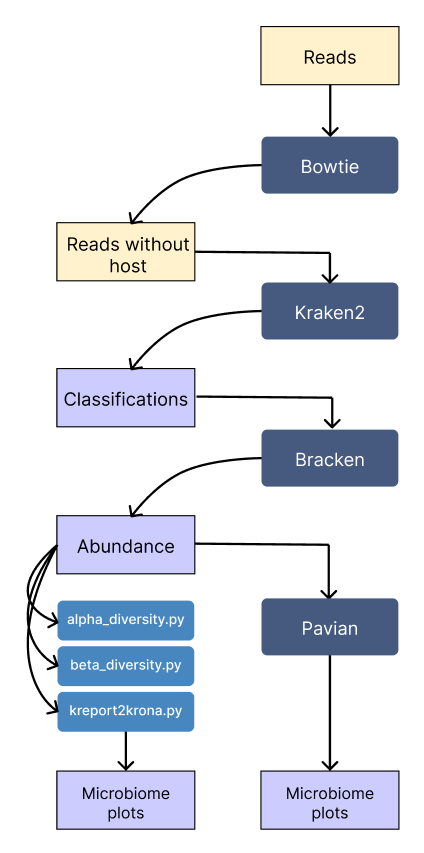
\includegraphics[scale=0.5]{images/shotgun_workflow.png}
                \caption{The shotgun workflow}
                \small Relative to the previous workflow, the updated procedure incorporates Bowtie2 at the outset to eliminate host DNA from the reads. Following the classification by Kraken 2, the data is processed by Bracken to yield abundance information. This information is subsequently visualized using Pavian and KrakenTools, as depicted by the three scripts presented in the figure.
                \label{fig:methods:new_shotgun_workflow}
            \end{figure}
            
        The process of the shotgun workflow illustrated in figure \ref{fig:methods:new_shotgun_workflow} commences with the removal of human host DNA using Bowtie2. For some datasets collected, the host DNA is already removed, then this step can be skipped.

        Then it is followed by the taxonomic classification of sequencing reads using \tool{Kraken2}\cite{wood2019improved}. Each read is then allocated to a taxonomic group (species, genus, or higher-level taxa). The database used here is Standard plusPFP (Standard plus protozoa, fungi, and plant) version 2022-06-07. Optionally a report can be generated showing the aggregate counts of each classified result.
        
        And then subsequent step involves calculating the relative abundance of different species within the sample. \tool{Bracken} was devised to function alongside \tool{Kraken 2} for species abundance computation, utilizing the classification results from \tool{Kraken 2}. \tool{Bracken} \cite{lu2017bracken} then processes the classified read counts and estimates the abundance of each taxon in the sample.
        
        In the final analysis, \tool{KrakenTools} and \tool{Pavian} \cite{breitwieser2020pavian} offer a comprehensive toolkit for downstream statistical analysis and visualization of the classification and abundance estimation outcomes.
        
        \tool{Pavian} can be employed to examine and visualize the sample to identify differences. In addition, \tool{alpha\_diversity.py} can be utilized to measure the diversity in a sample, and \tool{beta\_diversity.py} can be applied to compare diversity across samples. \tool{kreport2krona.py} can convert the Kraken report into the Krona format, which can be visualized using \tool{Krona} by generating a Krona plot.

          \tool{KrakenTools} are not available in the suite of Galaxy tools, hence there is a need to integrate them into the Galaxy EU instance. The process of doing so involves several steps:

            1. Construct the Wrappers
            
            \tool{Planemo} is a command-line utility employed in creating Galaxy and Common Workflow Language artifacts, which encompass tools, workflows, and training materials. The procedure commences with the command planemo tool\_init --id 'id' --name 'name', which generates an XML file containing significant tags such as requirements, command, inputs, outputs, and help.
            
            The requirements tag should include the necessary packages to execute the tool that requires wrapping. For \tool{KrakenTools}, this mainly pertains to Python.
            
            The command tag houses the command line necessary to operate the tool, comprising input files, parameters, and outputs. These options will subsequently be defined in the inputs and outputs sections.
            
            The inputs tag encompasses the tool's input, which will be displayed on the tool's page within Galaxy for users to select input files or parameters. The input encompasses several parameter types, including data, integer, float, and boolean values. Advanced tools may also permit the setting of conditional parameters.
            
            The outputs tag involves the tool's output, which should also be encompassed within the commands.
            
            The help tag should offer valuable information to assist new users in learning how to employ the tool.

            Proper configuration is essential for creating a user-friendly interface that facilitates easy understanding of the tool. This consideration is not only vital for the current workflow but also for all researchers utilizing the Galaxy platform.
            
            2. Construct Test Cases
            
            A proficient tool wrapper should include tests to ensure the smooth operation of the tool. These tests can also be set within the XML file. Multiple tests can be constructed, each involving example inputs and example outputs. 
            
            \tool{Planemo} utilizes the commands in the XML file to generate results using the inputs. If the generated result aligns with the anticipated outputs, it is declared that the tool is functioning correctly. All potential edge cases should be taken into account in these tests. Importantly, the example input and output files should not exceed 1MB in size.
            
            3. Submit the Pull Request on Tools-IUC
            
            Tools-IUC (https://github.com/galaxyproject/tools-iuc) is a GitHub repository that contains a selection of Galaxy repositories used in the Tool Shed (https://toolshed.g2.bx.psu.edu/). These repositories are maintained and developed by the Intergalactic Utilities Commission. Tools-IUC maintains high standards for Galaxy tools, further ensuring the smooth operation of the tool.
            
            4. Submit the Pull Request on Galaxy EU
            
            Following submission to Tools-IUC, this does not automatically make the tools usable. They must also be added to a Galaxy instance, in this case, Galaxy EU. Hence, a pull request should also be submitted to the Galaxy Europe. This is achieved by adding all the tool ids to the job\_conf.yml in the Galaxy infrastructure playbook, thereby instructing the Galaxy job dispatcher to pick up the tools.
            
            Finally, alpha\_diversity.py, beta\_diversity.py, and kreport2krona.py are integrated into the Galaxy EU instance and are prepared for use.

        
        \subsubsection{Evaluation of workflows}

            Despite the user-friendly features of the Galaxy platform, executing workflows on a large dataset, such as the more than 300 beer samples mentioned earlier, can be a ton of work. Fortunately, through the use of Bioblend, a Python library designed for interfacing with the Galaxy API, it is possible to automate the execution of workflows. The automation process shown in figure \ref{fig:methods:evaluation_of_workflows} is carried out through several discrete steps:
            
            \begin{figure}[H]
                \centering
                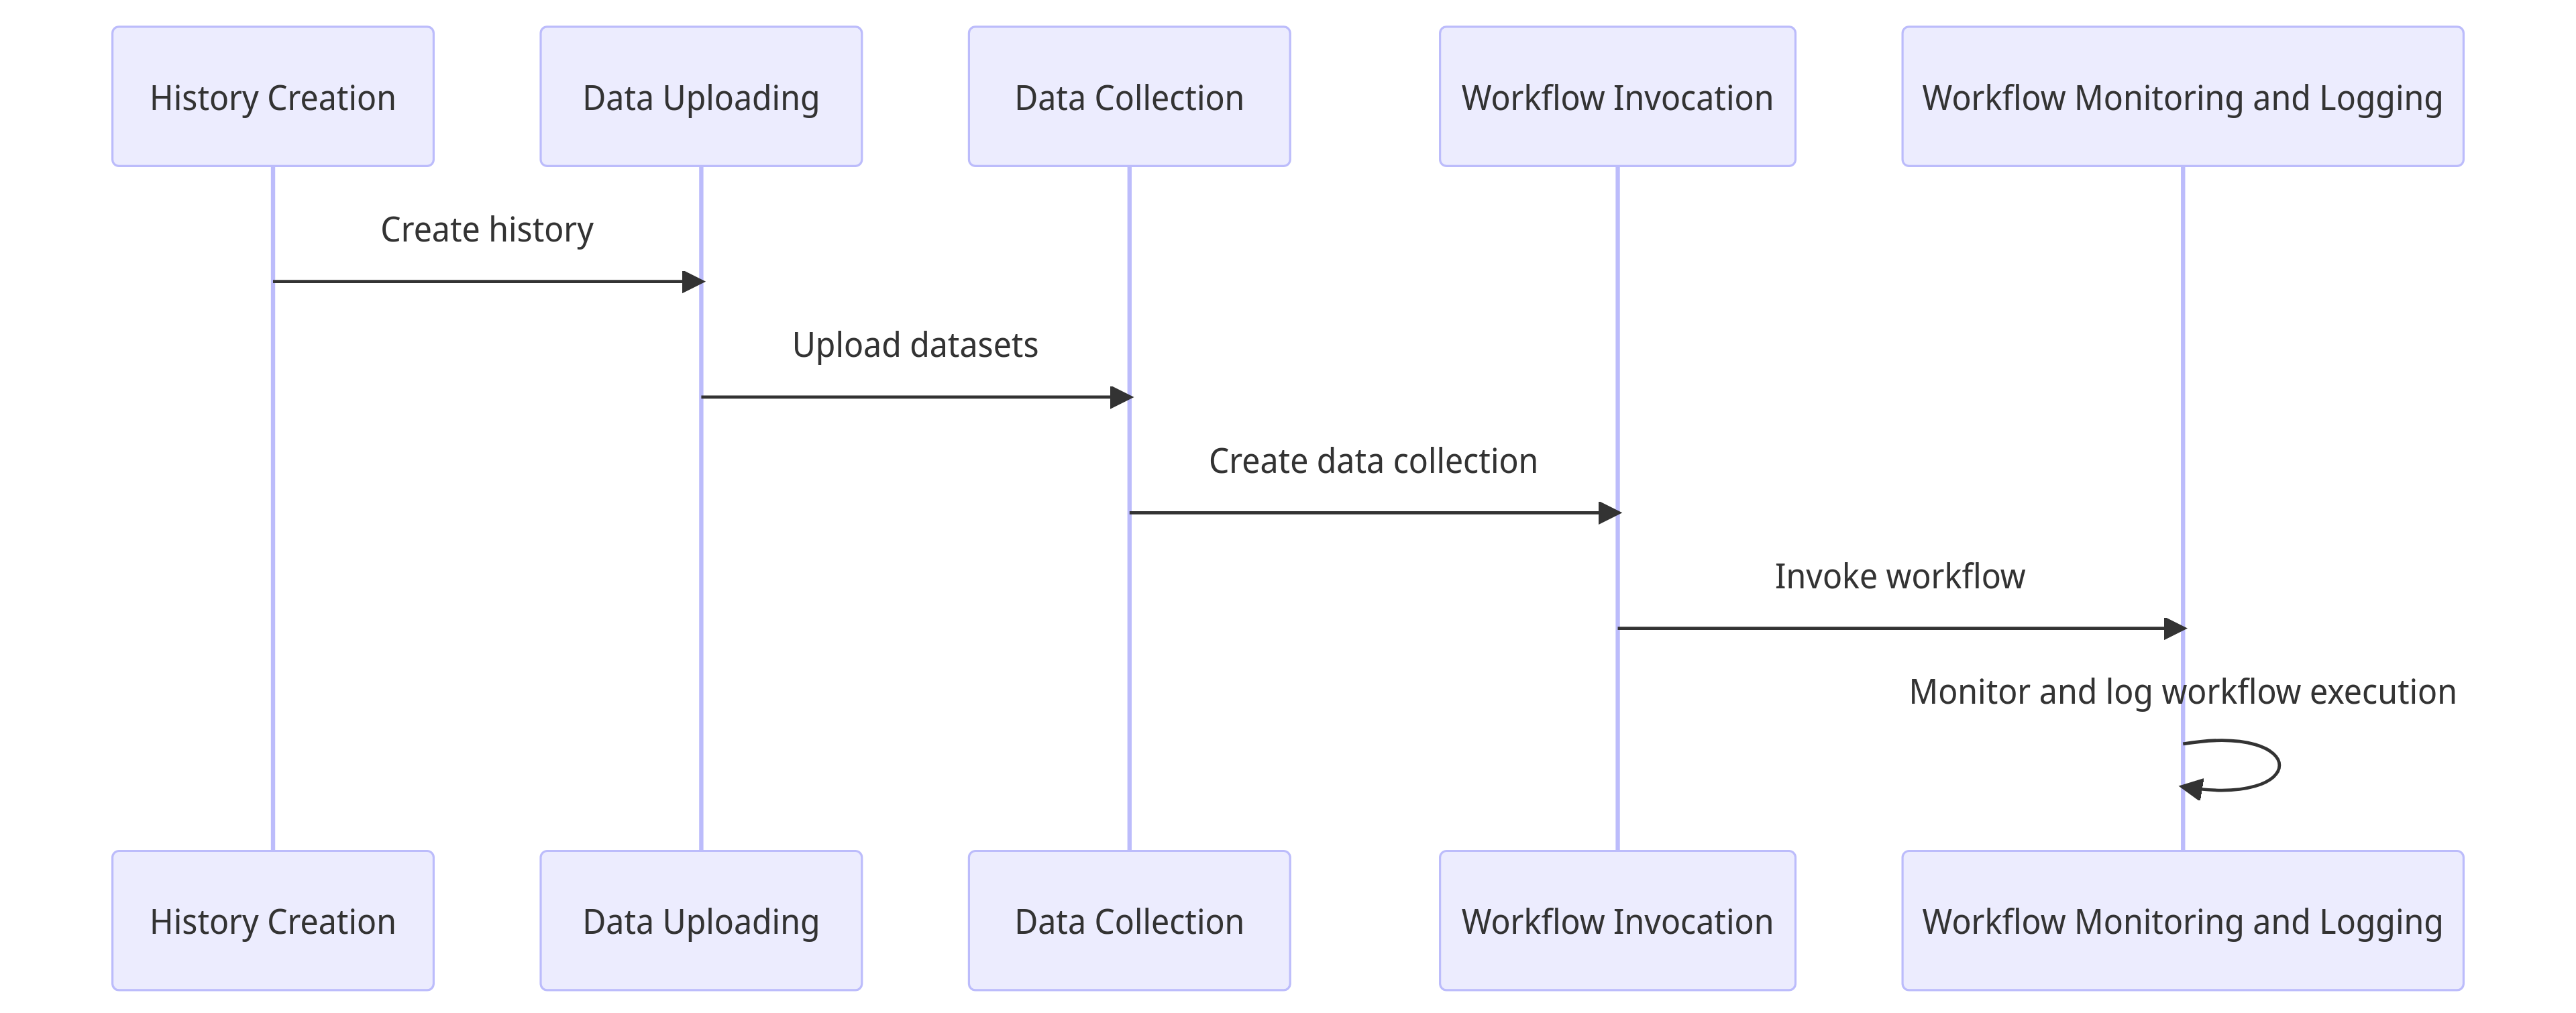
\includegraphics[scale=0.11]{images/evaluation_of_workflows.png}
                \caption{Automation of workflows execution}
                \label{fig:methods:evaluation_of_workflows}
                \small The figure illustrates the automation of workflow execution via Python scripts, leveraging Bioblend. The encompassed steps entail the creation of history, data upload procedures, formulation of data collection, the invocation of the workflow, and diligent workflow monitoring complemented by logging.
            \end{figure}   

            History Creation: In the Galaxy system, the concept of a 'history' denotes a unique computational environment that encapsulates specific datasets and analyses. For every distinct study, the script generates a new history, establishing an isolated workspace for data storage and manipulation. This new history is then associated with its corresponding project ID in a locally stored JSON file, providing easy access for future retrieval.
            
            Data Uploading: The next step in the process involves uploading the project's datasets to the newly created history. This is achieved by forming a single string of the dataset links, which is then uploaded through the upload\_dataset function. This function returns the result of the upload operation, which is further utilized in the subsequent steps. To ensure the robustness of the automation, the script actively monitors the status of the dataset upload operation. If the data is not yet available, the script pauses for a minute before rechecking, thereby preventing premature progression to the next steps.
            
            Data Collection: The datasets are then systematically paired if needed and organized into a Galaxy collection using the create\_paired\_dataset\_collection function. This preparation facilitates efficient downstream analyses by streamlining the data structure.
            
            Workflow Invocation: The datasets having been suitably prepared, the script proceeds to invoke the desired workflow. This is facilitated by mapping the datasets to the inputs of the workflow, identified by its unique ID. The workflow is then run on these datasets within the current history via the gi.workflows.invoke\_workflow function.
            
            Workflow Monitoring and Logging: Perhaps the most crucial step in this automated pipeline is monitoring the execution of the workflow. The updated monitor\_workflow\_execution function keeps track of the workflow status and logs it into a CSV file. This consistent tracking enables the prompt detection of potential issues and the successful completion of the workflow, thereby enhancing the reliability of the process.
            
            By doing these steps, it allows for the efficient handling and processing of multiple projects simultaneously and minimizes manual intervention and potential errors. The scripts for doing these steps are available here \url{https://github.com/YedilSerzhan/beer_microbiome/tree/main/data_plot_n_processing}.


            \subsubsection{Reproducibility analysis}

            This section describes the methodologies and tools used to examine workflow reproducibility, with a particular focus on the three previous studies chosen. I employed \tool{Python} programming language (version 3.9) and \tool{Jupyter Notebook} to conduct the analysis. 
            
            Python libraries \tool{Pandas}\cite{reback2020pandas}, \tool{Matplotlib}\cite{hunter2007matplotlib}, and \tool{Seaborn}\cite{Waskom2021} are utilized for data manipulation and visualization. \tool{Pandas} is a robust and widely used library that offers versatile data structures for efficient data manipulation and cleaning. \tool{Matplotlib} is a highly customizable plotting library that provides a vast array of tools to create high-quality figures for data visualization. \tool{Seaborn}, a statistical data visualization library built on \tool{Matplotlib}, streamlines the creation of informative and attractive plots.
            
            To assess the difference of diversity between original and reproduced data, I applied the Shapiro-Wilk test for normality and the paired-sample t-test, which were implemented using functions from the \tool{scipy.stats} module. The Shapiro-Wilk test is a widely used statistical method for determining if a given dataset is normally distributed. The paired-sample t-test, on the other hand, is employed to compare the means of two related groups, which is particularly useful for assessing the effects of different treatments on a given sample set. The \tool{shapiro} and \tool{ttest\_rel} functions from the \tool{scipy.stats}\cite{2020SciPy-NMeth} module were employed to conduct the Shapiro-Wilk test and paired-sample t-test, respectively. The metrics of the alpha diversity include Chao1, Shannon, and Simpson. Chao1 metric primarily estimates species richness, which is the number of different species present in a sample. Shannon Index encapsulates both species richness and evenness within a community. While also capturing species richness and evenness, the Simpson Index places more weight on the most abundant species.
            
    \subsection{Beer microbiome database: BeerMicroDB}

        The results generated from the analysis of beer data samples collected using the workflows mentioned above serve as the foundation for the beer microbiome database, MicroBeerDB.

        \subsubsection{Database implementation}

        
        \begin{figure}[H]
            \centering
            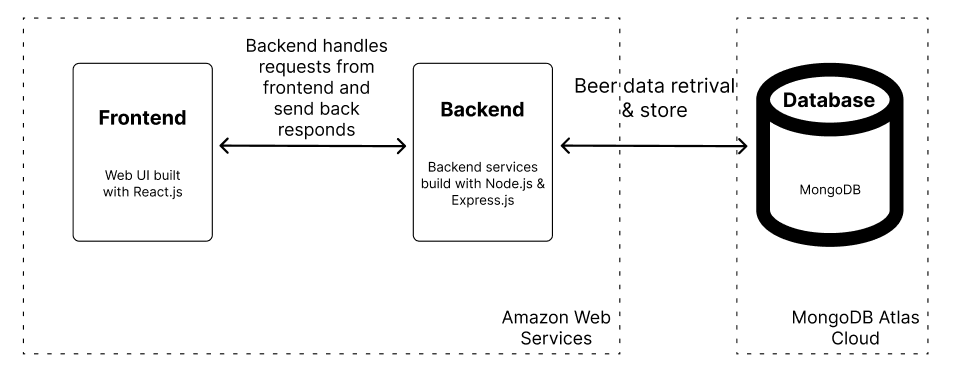
\includegraphics[scale=0.5]{images/system_architecture.png}
            \caption{The system architecture diagram of BeerMicroDB}
            \small The frontend of BeerMicroDB is constructed using React.js. Resources for this frontend are sourced from requests to the backend, developed with Express.js. This backend interfaces with a database established in MongoDB. Both the frontend and backend are deployed on Amazon Web Services, while the database resides on the MongoDB Atlas Cloud.
            \label{fig:methods:system_architecture}
        \end{figure}   

        The MicroBeerDB consists of 3 parts: 1. a frontend website built with React.js providing a web user interface. 2. Backend services built with Node.js and Express.js providing API services. 3. MongoDB hosted on MongoDB Atlas Cloud to store required data.

        \paragraph*{Frontend implementation}

            The frontend implementation of the Beer Microbiome Database website is primarily built using React, a powerful JavaScript library for constructing user interfaces, along with Material-UI, a popular React UI framework.

            \begin{figure}[H]
                \centering
                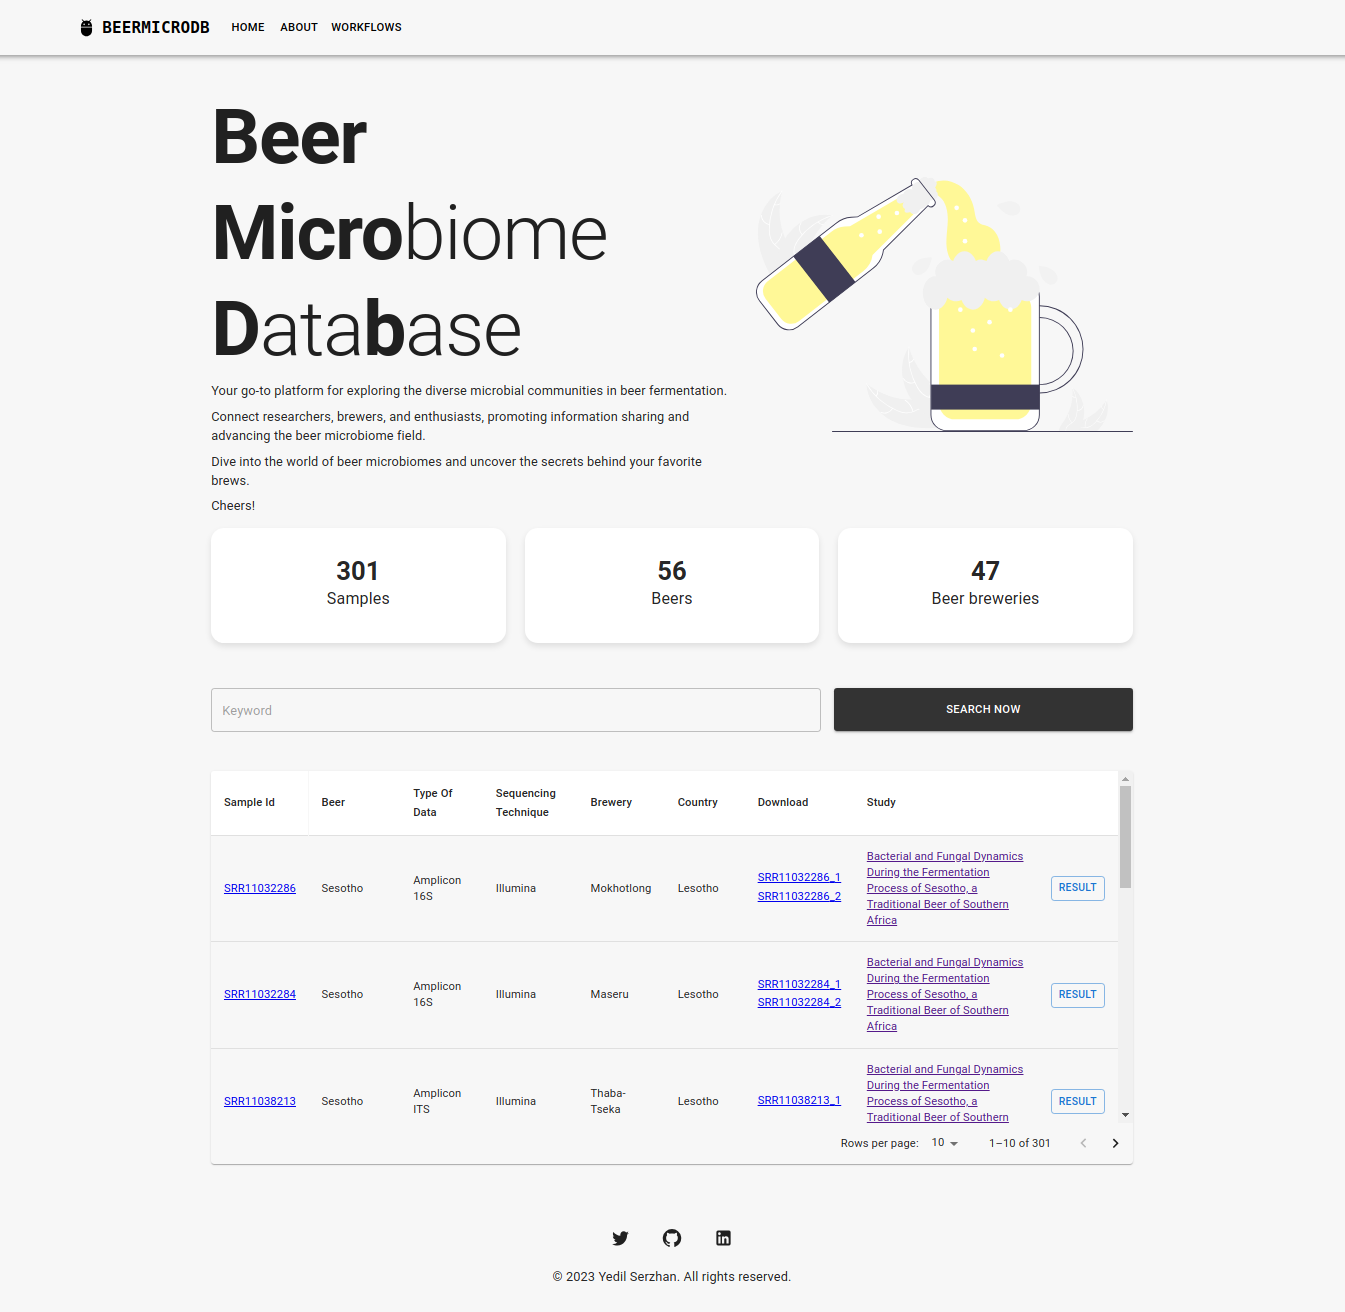
\includegraphics[scale=0.3]{images/home_page.png}
                \caption{BeerMicroDB Home page}
                \small The homepage features a welcoming and explanatory message accompanied by an image of beer at the top. This is followed by a section presenting statistics pertaining to BeerMicroDB. Further down, a search bar allows users to seek specific information, with the results displayed in a table format beneath it.
                \label{fig:methods:beermicrodb_home_page}
            \end{figure}  

            The Home page shown in figure \ref{fig:methods:beermicrodb_home_page} serves as the primary entry point to the application. Here, a combination of Material-UI components is used to create a visually appealing layout. The Home page contains a search bar, and a table constructed using Material-UI components displaying various microbiome samples. This page makes an asynchronous fetch request to a server upon mount to retrieve the microbiome sample data. This data is then managed using the useState and useEffect hooks from React to implement a search functionality, allowing users to filter through the microbiome samples based on their search criteria. The sample table includes pagination, offering a user-friendly way to navigate through potentially large sets of data. Each row in the table represents a single sample and provides a link to the study page that the sample belongs to. 

            The Study page, a dynamic component of the application, employs React Router's useParams hook to capture the study ID from the URL. This ID is subsequently used to dynamically import corresponding study results. This page shows the community profiling result at the species level for each sample belonging to the study.
            
            The About page delivers valuable insights about the project's purpose, context, methodologies, and data sources. The Workflows page exhibits the shotgun and metabarcoding sequencing workflow diagram, elucidating the process involved in analyzing the microbiome samples.
            
            All pages have a consistent layout and are equipped with a navigation bar and a Footer component, providing guidance to different components of the website. It utilizes the BrowserRouter, Routes, and Route components from the react-router-dom library to handle the navigation between different parts of the website.
                        
            In summary, the tech stack for the Beer Microbiome Database frontend implementation allows for the creation of dynamic, interactive web pages. And it provides a smooth user experience. The user interface is divided into distinct components, promoting the reusability and maintainability of the code. The frontend code base is available at \url{https://github.com/YedilSerzhan/beer_microbiome/tree/main/frontend}. 

        
        
        \paragraph*{Backend implementation}
        
            The backend is built with Express, a minimalistic and flexible Node.js web application framework, coupled with the Mongoose library for MongoDB \cite{banker2016mongodb}. 

            \begin{figure}[H]
                \centering
                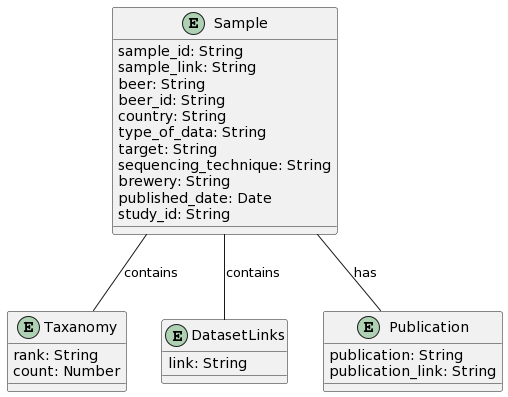
\includegraphics[scale=0.5]{images/db_model.png}
                \caption{Database models}
                \small In the MongoDB, the sample document model encompasses both metadata and the outcomes of microbiome analysis pertinent to each respective sample.
                \label{fig:methods:db_model}
            \end{figure}   
        
            The mongoose-based 'Sample' schema illustrated in figure \ref{fig:methods:db_model} stands as the cornerstone of our database model. This schema was carefully designed to accommodate a plethora of attributes intrinsic to the beer microbiome samples, such as 'sample\_id', 'beer', 'brewery', 'taxonomy', and more. Notably, 'taxonomy' is an array of objects, capturing information on various taxonomic ranks and their respective counts - a fitting representation of the complexity of microbiome data. In addition to these, the model carries metadata attributes including 'sequencing\_technique', 'country', 'published\_date', 'dataset\_links', and more, thereby encapsulating the diverse spectrum of data associated with each microbiome sample.
            
            The implementation of RESTful API operations is achieved through distinct route handlers for each HTTP method (GET, POST, PUT, DELETE). Each route corresponds to a specific action - obtaining all samples, getting a single sample, creating a new sample, updating an existing sample, and deleting a sample. The utilization of asynchronous functions in each route ensures non-blocking code execution.

            The backend code base is available at \url{https://github.com/YedilSerzhan/beer_microbiome/tree/main/backend}. 
                
        \subsubsection{Data ingestion}

        Data ingestion is the process of populating a database. In our case, we need to populate the results of workflows on the beer sample data to the microbiome database we are building.

        Firstly we perform data preprocessing on a DataFrame 'df' that contains the beer microbiome result. The taxonomy, dataset\_links, and publication related to the sample are objectified and saved to 'db\_ready.json', ready for ingestion.
                
        Then a code snippet initiates the later process by setting up a connection with the MongoDB database using the 'mongoose' library. Once the connection is established, the 'fs' (File System) module reads the 'db\_ready.json' file, containing the data to be populated. The JSON file is read asynchronously to prevent the blocking of subsequent operations.
        
        Each object in the JSON array is instantiated as a 'Sample' model, which is defined by the 'Sample' schema in Mongoose. This operation ensures that the data being saved adheres to the structure and validation rules defined in the schema. A save operation is then executed asynchronously on the instantiated 'Sample' model. If the save operation is successful, a console message confirming the ID of the saved record is printed. Otherwise, an error message is logged.
        
        In this way, the beer microbiome results are populated into the database. The scripts to do the data ingestion can be accessed at \url{https://github.com/YedilSerzhan/beer_microbiome/tree/main/backend/data}.
        